\documentclass{article}

\usepackage{a4}
\usepackage{amsmath}
\usepackage{amssymb}
\usepackage{ctex}
\usepackage{booktabs}
\usepackage{graphicx}
\usepackage{float}
\usepackage{hyperref}
\usepackage{enumitem}
\usepackage{array}
\usepackage{fvextra}
\usepackage{xurl}

\hypersetup{colorlinks=true,linkcolor=black,urlcolor=blue,citecolor=black}
\RecustomVerbatimEnvironment{verbatim}{Verbatim}{
  breaklines=true,
  breakanywhere=true,
  fontsize=\small
}
\newcommand{\TraceSize}{\fontsize{5}{6.05}\selectfont}
\newcommand{\tracecol}[2]{%
  \begin{minipage}[t]{0.492\textwidth}
    \centering{\small #1}\par\vspace{0.25em}
    \VerbatimInput[fontsize=\TraceSize,breaklines=true,breakanywhere=true]{#2}
  \end{minipage}%
}
\newcommand{\tracepair}[2]{%
  \par\noindent\tracecol{gettrace}{#1}\hfill\tracecol{mycpu}{#2}\par
}
\setlist[itemize]{nosep,leftmargin=1.8em}
\setlist[enumerate]{nosep,leftmargin=1.8em}

\title{计算机体系结构\\实验2\\乘除、分支跳转与访存指令的添加}
\author{鲁昕宁 \quad 2414015}
\date{2026年10月23日}
\begin{document}

\maketitle
\begin{center}
\begin{tabular}{ll}
GitHub仓库 & \parbox[t]{0.72\textwidth}{\url{SidneyLu/Computer-Architecture-NKU-CS/tree/master/lab2}} \\[0.6em]
班号 & \underline{0964} \\[0.6em]
授课教师 & \underline{董前琨} \\[0.6em]
\end{tabular}
\end{center}

\newpage

\section{实验目标}
本实验接着实验1带前递的五级流水线，完成《CPU设计实战》第5章和第6章。
CPU 仍是 \texttt{mycpu\_verify/rtl/myCPU}。

\begin{enumerate}
  \item 补齐算术、逻辑、变量移位，以及 \texttt{MULT}/\texttt{MULTU}/\texttt{DIV}/\texttt{DIVU}
        和 HI/LO 的读写，使 \texttt{func\_lab6} 的 42 个功能点与参考轨迹一致。
  \item 补齐 \texttt{J}、条件分支、\texttt{JALR}，以及字节、半字和非对齐的
        \texttt{LWL}/\texttt{LWR}/\texttt{SWL}/\texttt{SWR}，使 \texttt{func\_lab7}
        的 68 个功能点通过。
\end{enumerate}

乘法和除法用 Vivado 的 \texttt{mult\_gen}、\texttt{div\_gen}。
前递和 load-use 停顿沿用实验1。没有实验箱，结论以仿真波形和 trace 对比为准。

\section{实验原理}
流水线、阻塞和前递已经写在实验1里。下面是这次新增的立即数扩展、HI/LO 和按字节访问存储器。

\subsection{两种立即数扩展}
\texttt{ADDI}、\texttt{SLTI}、\texttt{SLTIU}、访存偏移和 \texttt{LUI} 的低 16 位按符号扩展。
\texttt{ANDI}、\texttt{ORI}、\texttt{XORI} 单独零扩展。逻辑立即数最高位为 1 时，
符号扩展会把高 16 位填成 \texttt{ffff}。

\texttt{SLTIU} 的立即数仍做符号扩展，比较按无符号进行。
负数扩展后接近 $2^{32}$，无符号比较时大于绝大多数 32 位操作数。

\subsection{HI/LO 与多周期乘除}
\texttt{MULT}/\texttt{MULTU} 把 64 位积的高半写入 HI、低半写入 LO，
\texttt{DIV}/\texttt{DIVU} 把商写入 LO、余数写入 HI，余数的符号与被除数相同。
这四条指令不写通用寄存器。\texttt{MFHI}/\texttt{MFLO} 把 HI 或 LO 当作该指令的写回数据，
\texttt{MTHI}/\texttt{MTLO} 用 \texttt{rs} 覆盖 HI 或 LO。

乘法器流水级数为 1，结果再打一拍后采样，所以一条乘法在执行级占两拍。
除法器有符号延迟 36 拍、无符号延迟 34 拍。结果未到时 \texttt{es\_ready\_go} 为 0，
后续指令留在译码级。除法器的 \texttt{tvalid} 只在进入执行级后的一拍拉高；
每个时钟都保持为 1 时，除法会重新开始。测试程序不覆盖溢出例外和除零。

\subsection{部分字与非对齐拼接}
数据 RAM 按字寻址，\texttt{addr[17:2]} 选字，\texttt{addr[1:0]} 选字节。
小端下 \texttt{wen[0]} 对应 \texttt{[7:0]}。
\texttt{LB}/\texttt{LBU}/\texttt{LH}/\texttt{LHU} 在访存级抽出字节或半字再扩展，
旁路出去的是扩展后的值。\texttt{SB}/\texttt{SH} 只打开对应的写使能，
写数据把同一个字节或半字复制到整个字上，写使能关掉的字节保持原值。

\texttt{LWL}/\texttt{LWR} 用 \texttt{rt} 的旧值和内存中的字拼接。
旧值只在译码级读一次（含前递），然后锁存到访存级。
小端、地址低两位为 $k$ 时：

\begin{center}
\begin{tabular}{lll}
\toprule
$k$ & \texttt{LWL} & \texttt{LWR} \\
\midrule
0 & \texttt{\{mem[7:0], rt[23:0]\}} & \texttt{mem} \\
1 & \texttt{\{mem[15:0], rt[15:0]\}} & \texttt{\{rt[31:24], mem[31:8]\}} \\
2 & \texttt{\{mem[23:0], rt[7:0]\}} & \texttt{\{rt[31:16], mem[31:16]\}} \\
3 & \texttt{mem} & \texttt{\{rt[31:8], mem[31:24]\}} \\
\bottomrule
\end{tabular}
\end{center}

\texttt{BGEZAL}/\texttt{BLTZAL} 无论条件是否成立都写 \texttt{\$31 = PC+8}。
条件只决定下一条（延迟槽）之后从哪里取指。

\section{实验过程}
\subsection{IP 与存储器}
乘法器用两个 \texttt{mult\_gen}：有符号和无符号各一个，32$\times$32，LUT，
流水级数 1，端口是 \texttt{CLK}、\texttt{A}、\texttt{B}、\texttt{P[63:0]}。
除法器用两个 \texttt{div\_gen}，Radix2，操作数 32 位，输出带余数，
不检测除零，没有 \texttt{tready} 和复位。有符号延迟 36，无符号延迟 34。
商在 \texttt{tdata[63:32]}，余数在 \texttt{tdata[31:0]}。
乘法器则是高 32 位进 HI、低 32 位进 LO。

\texttt{inst\_ram.vhd} 是 IP 生成的只读文件。换程序要改 \texttt{inst\_ram.xci}
里的 COE，并对锁定的旧 IP 先 \texttt{upgrade\_ip}，再重新生成仿真文件。
\texttt{func\_lab6} 与 \texttt{func\_lab7} 的 coe 放在 \texttt{CPU\_CDE/soft/}。
\texttt{cpu132\_gettrace} 跑完后得到 \texttt{golden\_trace.txt}，
\texttt{mycpu} 的 testbench 按写回逐条比较。

\subsection{func\_lab6}
42 个功能点一次通过。同一序号上 \texttt{mycpu} 都更早到达：
乘除期间执行级停等，其余指令沿用实验1的前递，整段仿真短于参考 CPU。
逐点记录见第~\ref{sec:trace}~节。

\subsection{func\_lab7 与 LWR}
换成 \texttt{func\_lab7} 的 COE 后，第 1 到 63 点通过，第 64 点 \texttt{LWR} 第一次不一致：
\begin{verbatim}
reference: PC = 0xbfc9a264, wnum = 0x02, wdata = 0xca5c0495
mycpu    : PC = 0xbfc9a264, wnum = 0x02, wdata = 0xf15c0495
\end{verbatim}
该指令是 \texttt{lwr \$v0,-16999(\$at)}，地址低两位为 1。
内存字是 \texttt{5c049582}，\texttt{\$v0} 的旧值是 \texttt{ca18f110}。
正确拼接是 \texttt{\{rt[31:24], mem[31:8]\} = ca5c0495}。
原先把 \texttt{rt[31:8]} 与 \texttt{mem[31:8]} 接成 48 位，
Verilog 截断后高字节变成 \texttt{f1}。按上表的位宽改完后重新仿真，
68 个功能点通过，记录见第~\ref{sec:trace}~节。
延迟槽测试在这次修改之前已经通过，分支目标仍用实验1的 \texttt{fs\_pc + offset}。

\section{关键代码}
下面各段对应译码控制、HI/LO、模块级封装和部分字访存。

\subsection{译码：扩展、链接和乘除}
零扩展单独用 \texttt{src2\_is\_zimm}。链接类指令把 \texttt{PC} 和常数 8 送进 ALU，
目标寄存器是 \texttt{\$31}；\texttt{JALR} 用 \texttt{rd}。
乘除和 \texttt{MTHI}/\texttt{MTLO} 不写通用寄存器。
\begin{verbatim}
assign src2_is_imm  = inst_addiu | inst_addi | inst_slti | inst_sltiu
                    | inst_lui | inst_load | inst_store;
assign src2_is_zimm = inst_andi | inst_ori | inst_xori;
assign src1_is_pc   = inst_jal | inst_jalr | inst_bgezal | inst_bltzal;
assign src2_is_8    = inst_jal | inst_jalr | inst_bgezal | inst_bltzal;
assign dst_is_r31   = inst_jal | inst_bgezal | inst_bltzal;
assign gr_we        = ~(inst_store | inst_beq | inst_bne | inst_jr | inst_j
                      | inst_bgez | inst_bgtz | inst_blez | inst_bltz
                      | inst_mult | inst_multu | inst_div | inst_divu
                      | inst_mthi | inst_mtlo);
\end{verbatim}
\texttt{BLTZAL} 的条件是 \texttt{rs[31]}，\texttt{BGEZ} 是 \texttt{\textasciitilde rs[31]}。
条件不成立时 \texttt{br\_taken} 为 0，但 \texttt{gr\_we} 仍为 1，\texttt{\$31} 照常写回。

\subsection{HI/LO}
乘法器输出打一拍后采样。除法只在进入执行级的下一拍拉高一次 \texttt{tvalid}。
商进 LO，余数进 HI。\texttt{MFLO} 的写回数据取 LO。
\begin{verbatim}
assign es_ready_go = (es_is_mul | es_is_divop) ? md_ready : 1'b1;

if (es_valid && es_is_divop && div_accepted && div_vout && !md_ready) begin
    lo       <= div_dout[63:32];
    hi       <= div_dout[31:0];
    md_ready <= 1'b1;
end
if (es_valid && es_is_mul && !md_ready) begin
    if (!mul_seen) mul_seen <= 1'b1;
    else begin
        hi <= mul_res[63:32];
        lo <= mul_res[31:0];
        md_ready <= 1'b1;
    end
end
assign es_wb_data = es_is_mfhi ? hi : es_is_mflo ? lo : alu_result;
\end{verbatim}

\subsection{模块级封装}
\label{sec:mdwrap}
\texttt{mul\_tb}、\texttt{div\_tb} 的端口与 IP 不同。\texttt{mul.v}、\texttt{div.v}
把同一组核接到测试台上。两个乘法器每个时钟都在计算，
\texttt{mul\_signed} 打一拍后再选择结果，与 IP 的输出寄存器对齐。复位期间 \texttt{result} 保持 0。
\begin{verbatim}
always @(posedge mul_clk) begin
    if (!resetn) begin
        en       <= 1'b0;
        signed_r <= 1'b0;
    end
    else begin
        en       <= 1'b1;
        signed_r <= mul_signed;
    end
end
assign result = (!en)    ? 64'd0 :
                signed_r ? p_signed :
                           p_unsigned;
\end{verbatim}
除法在 \texttt{div} 为 1 且尚未接受时，把 \texttt{fire} 拉高一拍，
只送给 \texttt{div\_signed} 选中的核。
\texttt{signed\_hold} 记下符号，\texttt{complete} 取该核的 \texttt{dout\_tvalid}。
商在 \texttt{[63:32]}，余数在 \texttt{[31:0]}。
\begin{verbatim}
assign fire = resetn && div && !accepted;

div_gen_signed_0 u_signed (
    .s_axis_divisor_tvalid  (fire && div_signed),
    .s_axis_dividend_tvalid (fire && div_signed),
    ...
);
div_gen_unsigned_0 u_unsigned (
    .s_axis_divisor_tvalid  (fire && !div_signed),
    .s_axis_dividend_tvalid (fire && !div_signed),
    ...
);
assign s        = dout[63:32];
assign r        = dout[31:0];
assign complete = signed_hold ? vout_s : vout_u;

always @(posedge div_clk) begin
    if (!resetn) begin
        accepted    <= 1'b0;
        signed_hold <= 1'b0;
    end
    else if (!div)
        accepted <= 1'b0;
    else if (!accepted) begin
        accepted    <= 1'b1;
        signed_hold <= div_signed;
    end
end
\end{verbatim}

\subsection{字节写使能与 LWR}
\begin{verbatim}
assign st_wen = (es_mem_op == `MEM_SW) ? 4'b1111 :
                (es_mem_op == `MEM_SB) ? (4'b0001 << ea) :
                (es_mem_op == `MEM_SH) ? (ea[1] ? 4'b1100 : 4'b0011) :
                ...
assign data_sram_wen = es_valid ? st_wen : 4'h0;

(ms_mem_op == `MEM_LWR && ea == 2'd1) ? {ms_rt_value[31:24], mem_word[31:8]} :
(ms_mem_op == `MEM_LWR && ea == 2'd2) ? {ms_rt_value[31:16], mem_word[31:16]} :
(ms_mem_op == `MEM_LWR && ea == 2'd3) ? {ms_rt_value[31:8],  mem_word[31:24]} :
\end{verbatim}
\texttt{ea == 0} 的 \texttt{LWR} 以及 \texttt{LWL} 的 \texttt{ea == 3} 直接取 \texttt{mem\_word}。

\section{实验结果}
\subsection{功能点对比}
\label{sec:trace}
仿真控制台每隔约 10\,\textmu s 打印一行 \texttt{Test is running}。
下面保留功能点通过行和结束行。左栏是 \texttt{cpu132\_gettrace}，右栏是 \texttt{mycpu}，同一行是同一个功能点。
\texttt{gettrace} 结束时打印 \texttt{gettrace end!}，表示 \texttt{golden\_trace.txt} 已经写好；
\texttt{mycpu} 结束时打印 \texttt{----PASS!!!}，表示写回与这条轨迹一致。

\texttt{func\_lab6} 两边都到第 42 点。\texttt{gettrace} 在 1194255\,ns 结束，
\texttt{mycpu} 在 1077765\,ns 结束。

\tracepair{logs/gettrace_lab6.txt}{logs/mycpu_lab6.txt}

\texttt{func\_lab7} 两边都到第 68 点。\texttt{gettrace} 在 1835885\,ns 结束，
\texttt{mycpu} 在 1645135\,ns 结束。第 42 点仍是 1077305\,ns，与单独运行 \texttt{func\_lab6} 相同。
前 34 点两边相差不超过 34.3\,\textmu s。除法所在的第 35、36 点耗时接近；
第 37 点乘法之后差距拉开，到第 42 点为 0.116\,ms，到第 68 点为 0.191\,ms。

\tracepair{logs/gettrace_lab7.txt}{logs/mycpu_lab7.txt}

\begin{center}
\begin{tabular}{lrr}
\toprule
程序 & \texttt{mycpu} 结束 & \texttt{gettrace} 结束 \\
\midrule
\texttt{func\_lab6}（42 点） & 1.078\,ms & 1.194\,ms \\
\texttt{func\_lab7}（68 点） & 1.645\,ms & 1.836\,ms \\
\bottomrule
\end{tabular}
\end{center}

\subsection{乘除法器模块级测试}
封装见第~\ref{sec:mdwrap}~节。

\texttt{mul\_tb} 每拍更换一对随机操作数。
参考模型按 \texttt{mul\_signed} 把操作数扩成 33 位再相乘，并与打了一拍的输入比较。
10\,\textmu s 内 991 次比较全部为 \texttt{OK=1}。
有符号 $-2031628787 \times -1716266445 = 3486816315824152215$，
无符号 $4052285667 \times 1453815725 = 5891276624876713575$。

\texttt{div\_tb} 的原上限是 34 拍。无符号除法在第 34 拍给出 \texttt{complete}：
465\,ns 时 $2097015289 \div 3812041926$ 的商为 0、余数为 $2097015289$，
\texttt{s\_OK} 与 \texttt{r\_OK} 均为 1，同一拍测试台因到达上限而结束。
有符号除法在第 36 拍完成。上限改为 60 拍后，同一套随机激励在 50\,\textmu s 内完成 129 次除法，
商和余数全部与参考模型一致：无符号 67 次，每次 34 拍；有符号 62 次，每次 36 拍。
$-442812725 \div -217507098$ 的商为 2、余数为 $-7798529$；
$2087561720 \div -607297353$ 的商为 $-3$、余数为 $265669661$。
两例的余数符号都与被除数相同。

\subsection{波形}
波形从仿真 VCD 里截取短窗口，用 matplotlib 画出。时钟周期 10\,ns。
单周期脉冲的格子里不标十六进制，数值写在箭头旁。

\subsection{SLTIU}
\texttt{func\_lab7} 中 \texttt{bfc4ab28} 是 \texttt{sltiu \$v0,\$t0,-2967}。
\texttt{\$t0 = c255e3d8}，立即数符号扩展为 \texttt{fffff469}。
无符号比较成立，写回 1。若把立即数零扩展成 \texttt{0000f469}，
\texttt{c255e3d8} 更大，结果应是 0。图~\ref{fig:sltiu} 里访存级和写回都是 1。

\begin{figure}[H]
  \centering
  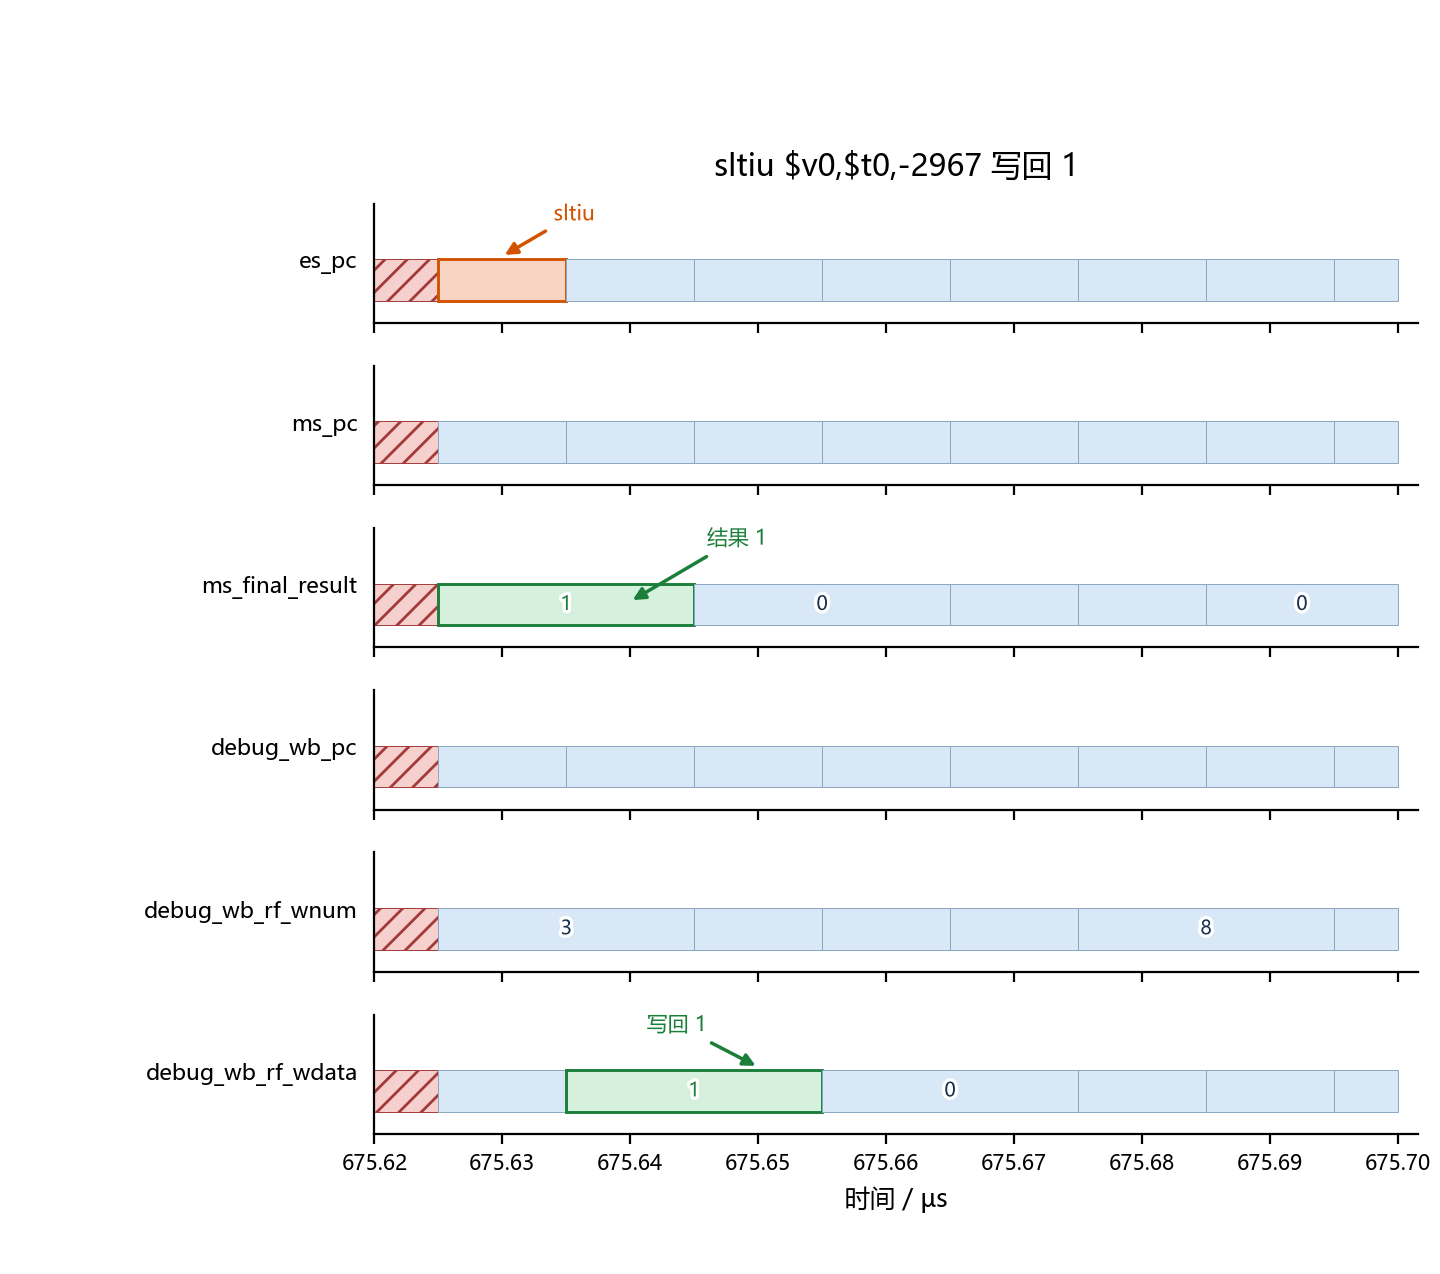
\includegraphics[width=\linewidth]{fig/sltiu.png}
  \caption{\texttt{sltiu} 在 675.63\,\textmu s 进入执行级，下一拍访存结果为 1，写回 1。}
  \label{fig:sltiu}
\end{figure}

\subsection{ANDI}
\texttt{bfc80c58} 是 \texttt{andi \$v0,\$t0,0x5e89}，\texttt{\$t0 = 4c23cdd4}。
零扩展后与出来是 \texttt{4c80}。同一立即数若符号扩展成 \texttt{ffff5e89}，
结果是 \texttt{4c234c80}。图~\ref{fig:andi} 的写回是 \texttt{4c80}，
和测试事先放入 \texttt{\$v1} 的参考值相同，随后的 \texttt{bne} 不跳转。

\begin{figure}[H]
  \centering
  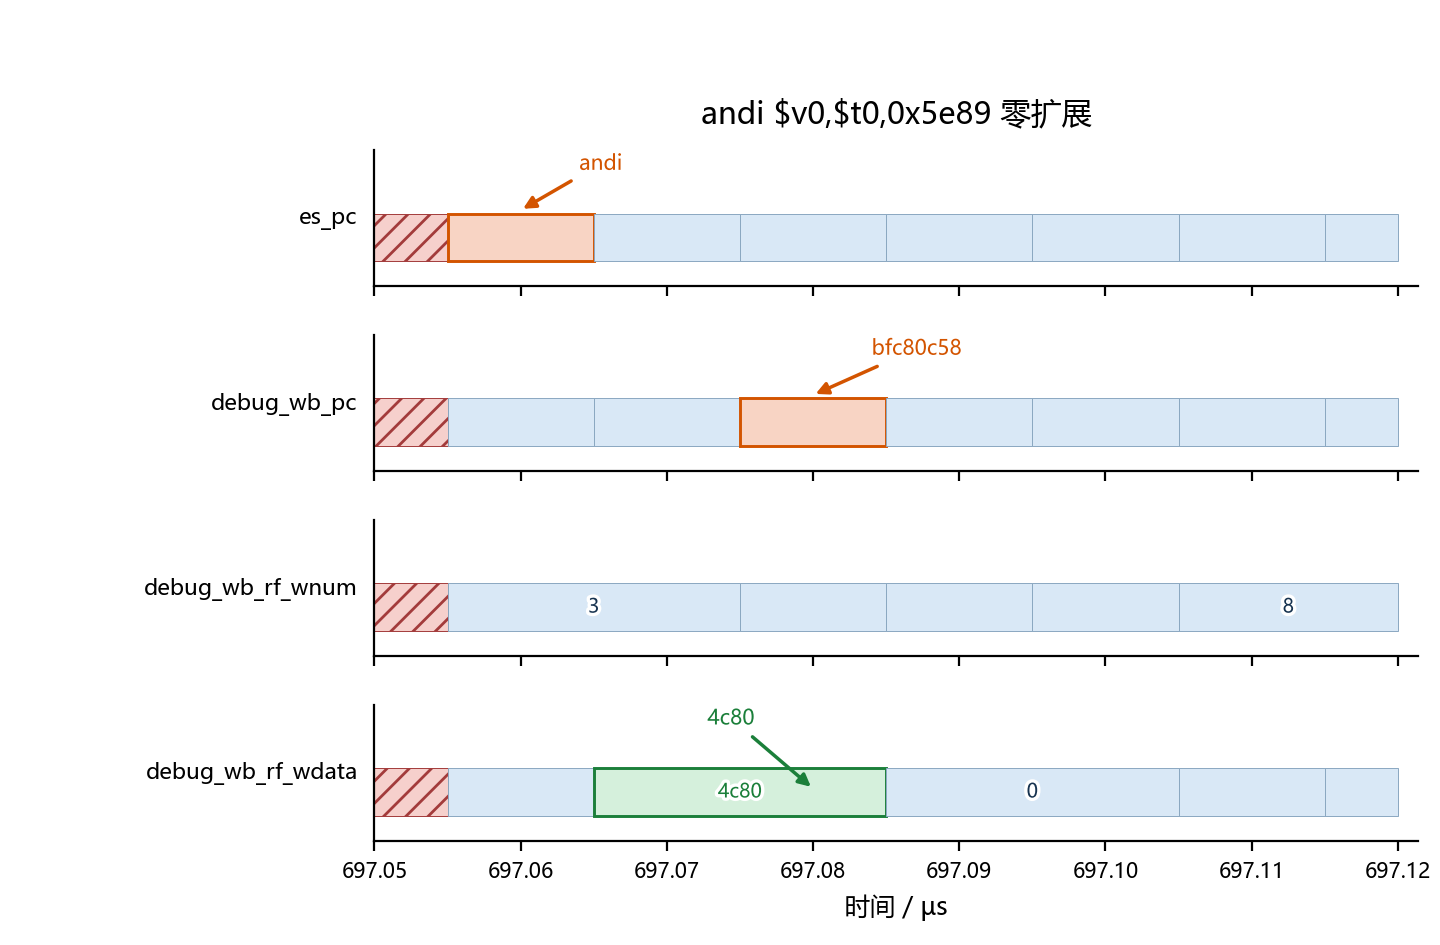
\includegraphics[width=\linewidth]{fig/andi.png}
  \caption{\texttt{andi} 写回 \texttt{4c80}。\texttt{debug\_wb\_pc} 为 \texttt{bfc80c58} 的那一拍与写回数据对齐。}
  \label{fig:andi}
\end{figure}

\subsection{MULT 与 MFLO}
\texttt{bfc85118} 的 \texttt{mult \$t0,\$t1} 中，\texttt{\$t0 = 45b90738}，\texttt{\$t1 = d70d64f0}。
执行级 PC 停在这条指令上，\texttt{es\_ready\_go} 低了两拍（20\,ns）。
993.675\,\textmu s HI 变成 \texttt{f4d903bb}，LO 变成 \texttt{a20a480}，执行级同时放行。
紧跟着的 \texttt{mflo \$s5} 把 LO 写入通用寄存器，见图~\ref{fig:mult}。
除法的停顿与此相同：有符号核 36 拍、无符号核 34 拍后 \texttt{dout} 有效，
\texttt{es\_ready\_go} 保持为 0，直到 HI/LO 写完。\texttt{func\_lab6} 的 n35--n42 已通过。

\begin{figure}[H]
  \centering
  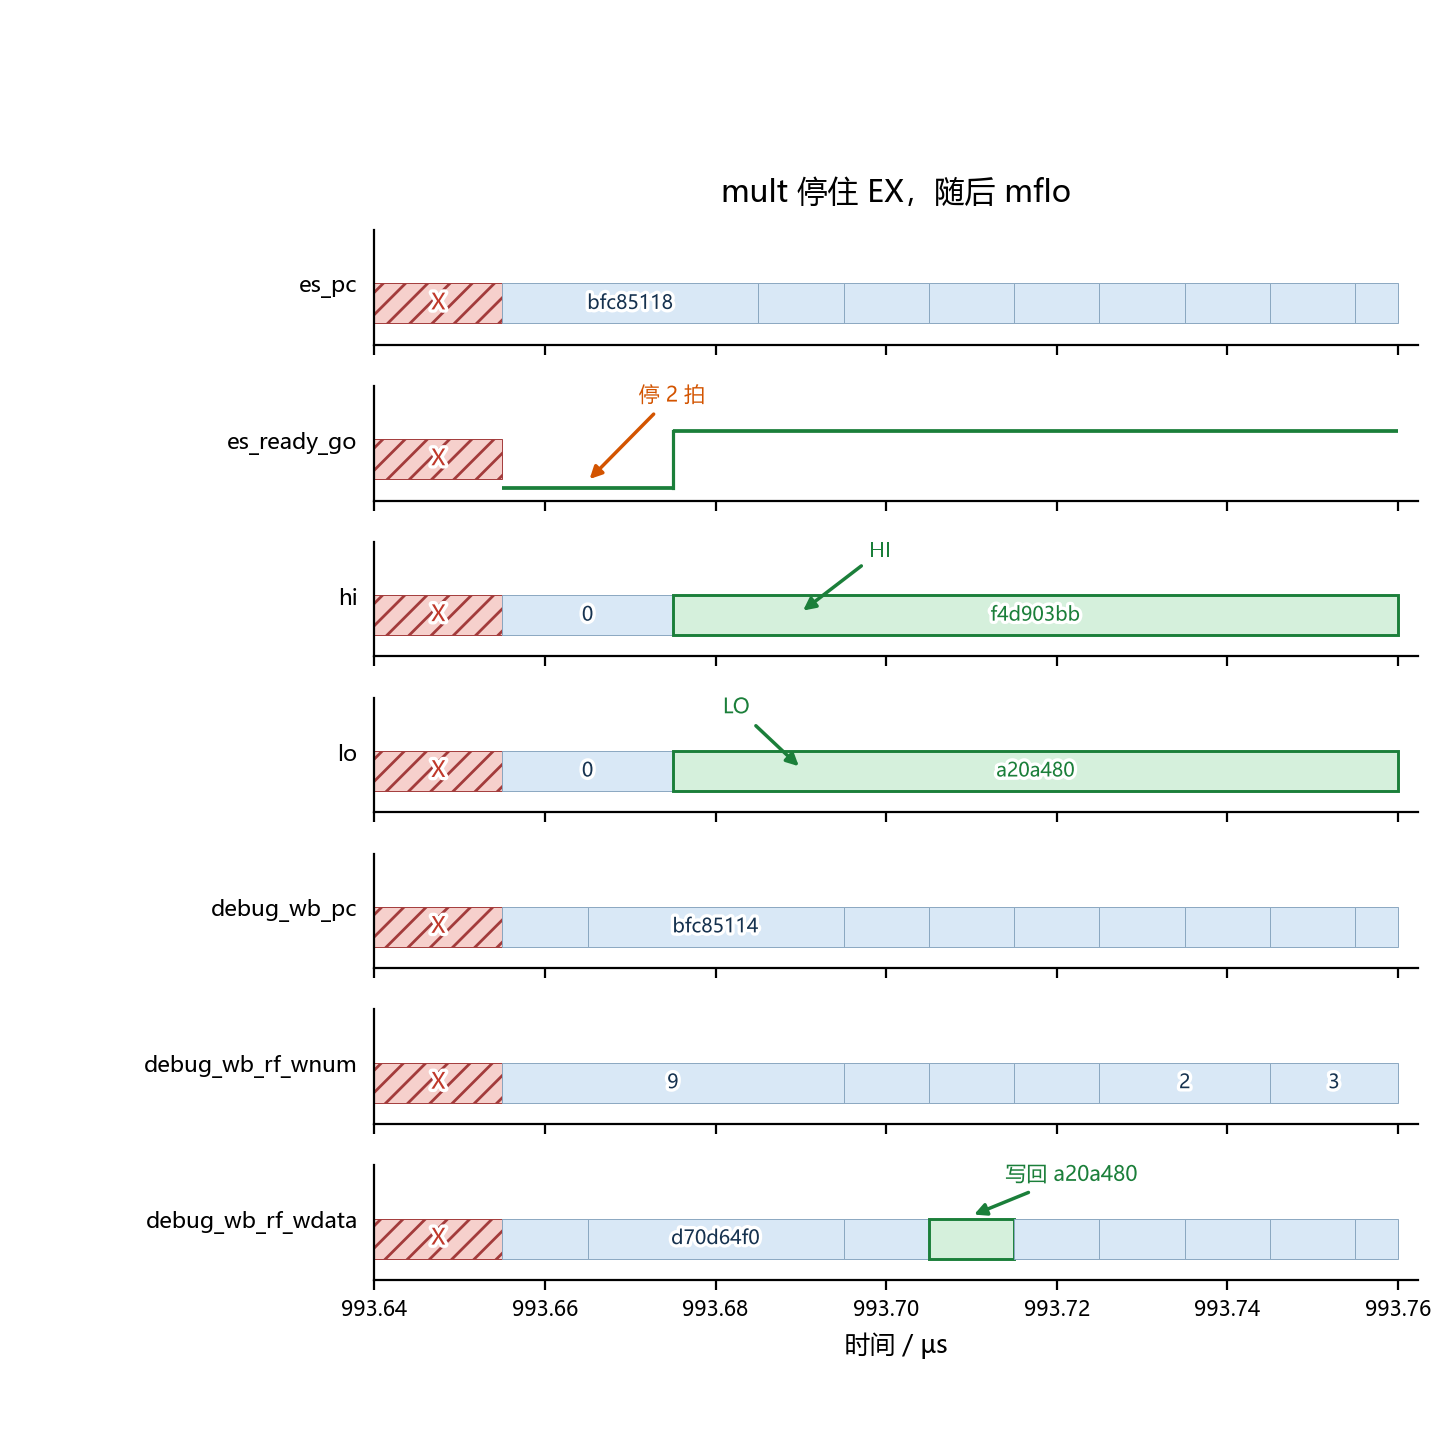
\includegraphics[width=\linewidth]{fig/mult.png}
  \caption{\texttt{mult} 停两拍后更新 HI/LO，\texttt{mflo} 写回 \texttt{a20a480}。}
  \label{fig:mult}
\end{figure}

\subsection{分支条件成立的 BGEZ}
\texttt{bfc60024} 是 \texttt{bgez \$t0, 目标}，\texttt{\$t0 = 44f2bff4}，条件成立。
图~\ref{fig:bgez} 里执行级先是这条分支，译码级是延迟槽 \texttt{bfc60028} 的 \texttt{nop}，
再下一拍 \texttt{ds\_pc} 变为 \texttt{bfc60000}，顺序地址 \texttt{bfc6002c} 被跳过。

\begin{figure}[H]
  \centering
  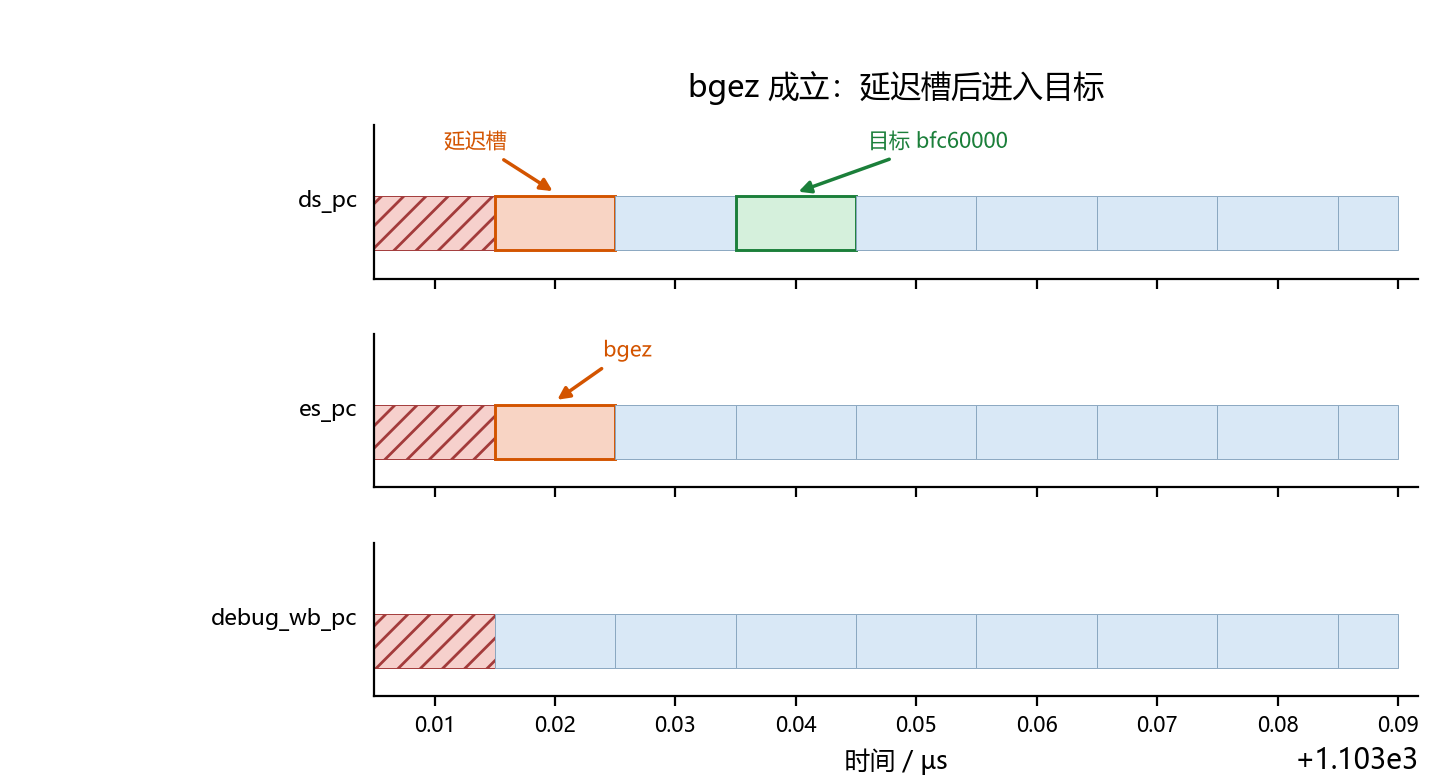
\includegraphics[width=\linewidth]{fig/bgez.png}
  \caption{分支条件成立的 \texttt{bgez}：延迟槽之后取目标 \texttt{bfc60000}。}
  \label{fig:bgez}
\end{figure}

\subsection{分支条件不成立的 BLTZAL}
\texttt{bfc40694} 是 \texttt{bltzal \$t0}，目标为 \texttt{bfc40670}。
\texttt{\$t0 = 655e408b}，符号位为 0，\texttt{br\_taken} 保持 0。
延迟槽 \texttt{bfc40698} 之后，\texttt{ds\_pc} 进入顺序地址 \texttt{bfc4069c}。
同一条指令把 \texttt{PC+8 = bfc4069c} 写入 \texttt{\$31}，见图~\ref{fig:bltzal}。

\begin{figure}[H]
  \centering
  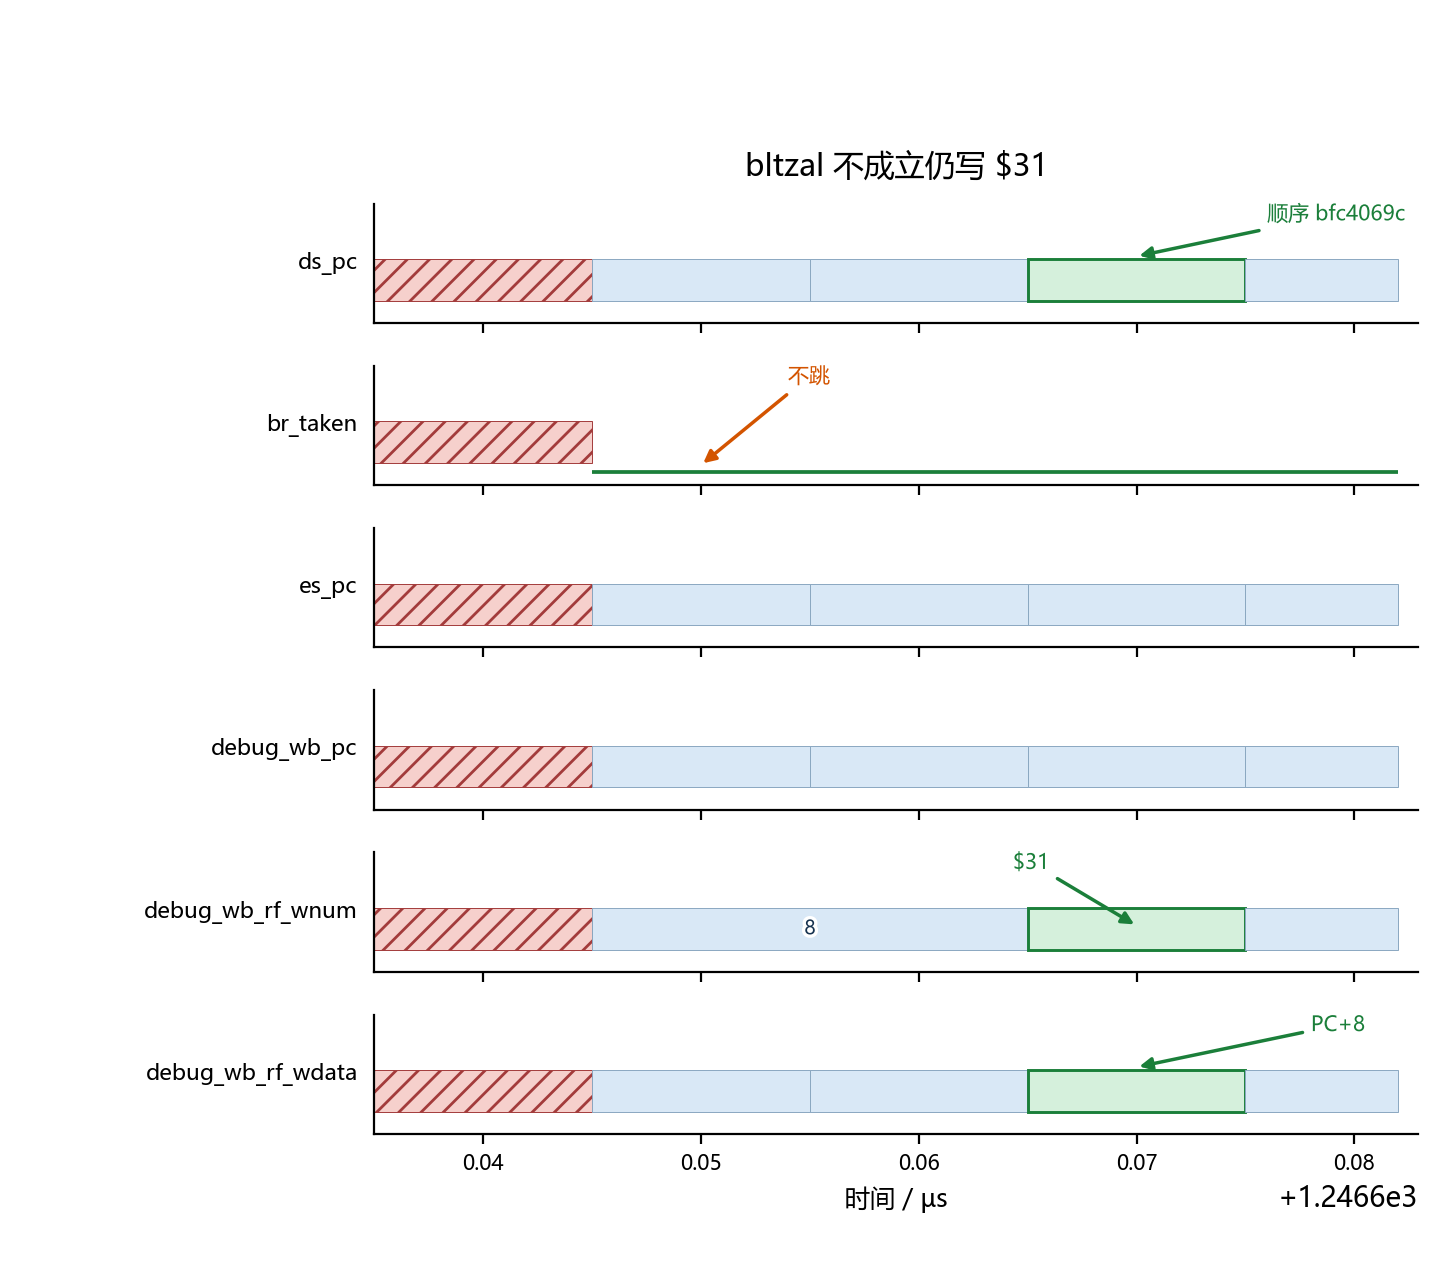
\includegraphics[width=\linewidth]{fig/bltzal.png}
  \caption{分支条件不成立的 \texttt{bltzal} 不改变 PC，写回寄存器号为 31，数据为 \texttt{PC+8}。}
  \label{fig:bltzal}
\end{figure}

\subsection{非对齐 LWR}
\texttt{bfc9a264} 就是前面写回不一致的那条 \texttt{lwr}。地址 \texttt{800dbd99} 的低两位为 1，
读回的字是 \texttt{5c049582}，锁存的 \texttt{rt} 旧值是 \texttt{ca18f110}。
拼接结果 \texttt{ca5c0495} 出现在访存级，并作为 \texttt{\$v0} 的写回，见图~\ref{fig:lwr}。
修正前这一拍写回的是 \texttt{f15c0495}。

同组 \texttt{LWL}（n63）在这次修正前已经通过。
例如 \texttt{bfc5beac} 的地址低两位为 2，按 \texttt{\{mem[23:0], rt[7:0]\}} 拼成
\texttt{e8d3ee80}，与测试参考值一致。

\begin{figure}[H]
  \centering
  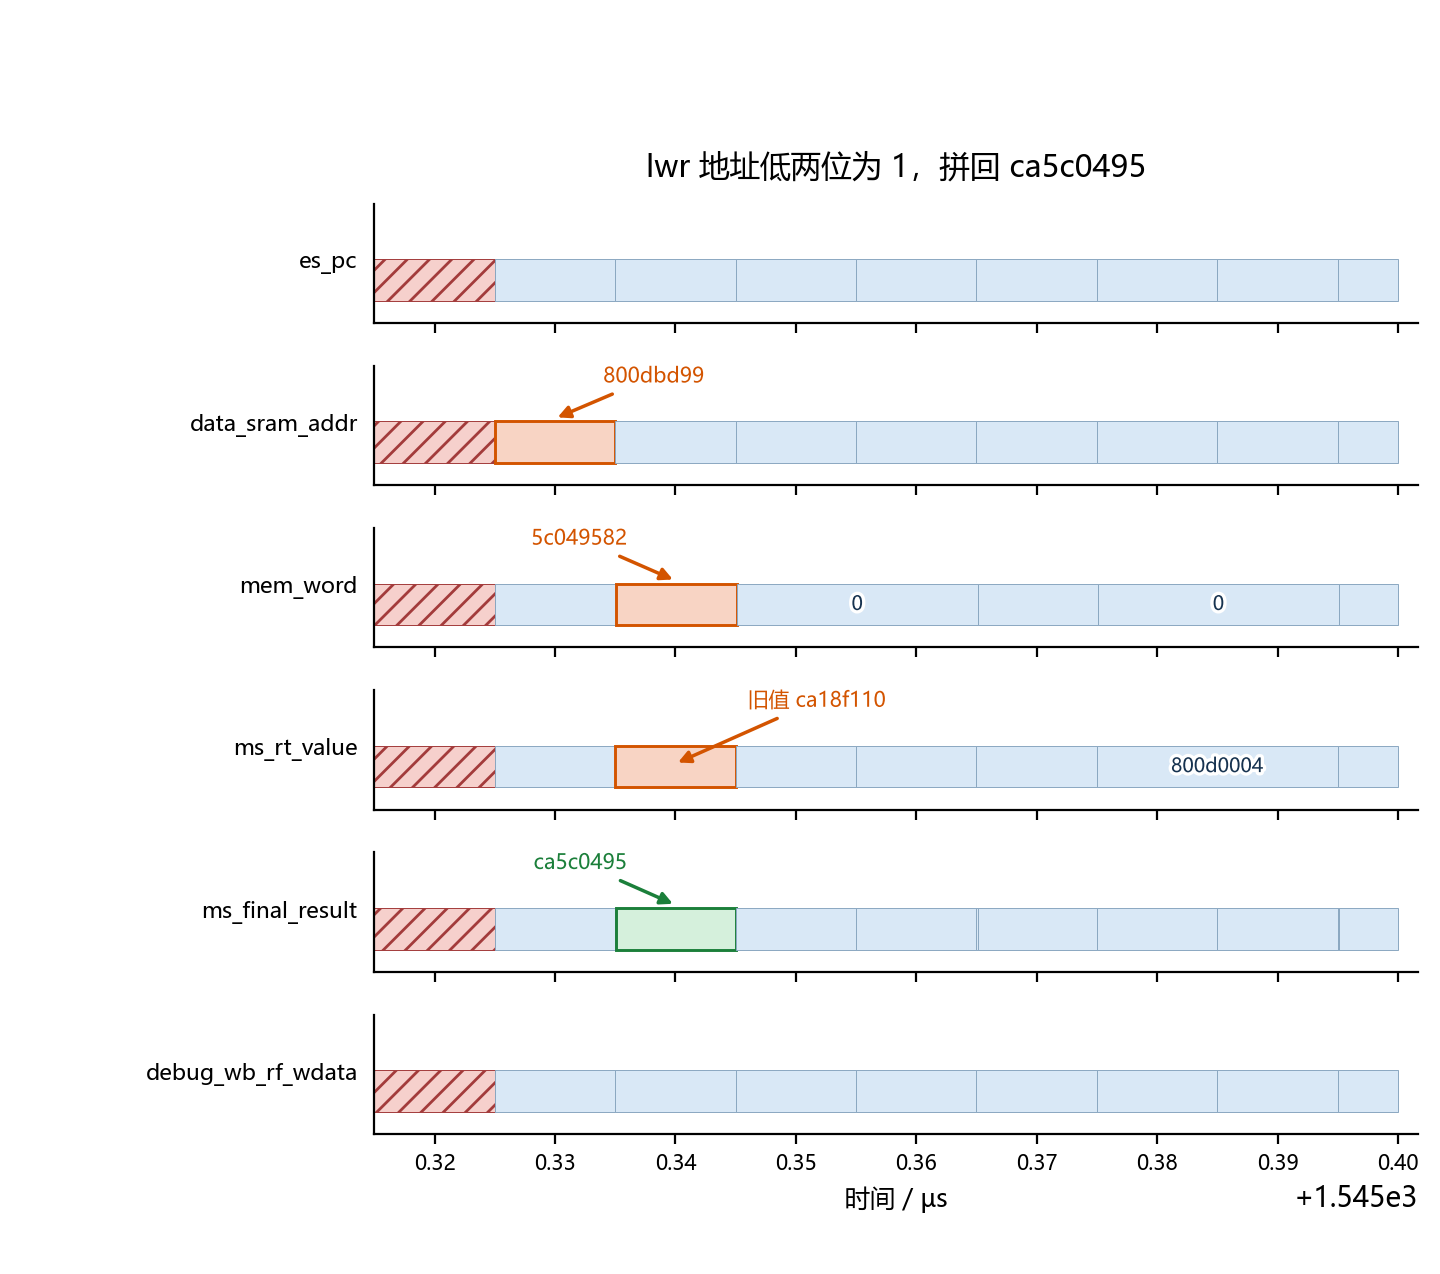
\includegraphics[width=\linewidth]{fig/lwr.png}
  \caption{\texttt{lwr}：地址低两位为 1，旧值高字节 \texttt{ca} 与内存 \texttt{[31:8]} 拼成 \texttt{ca5c0495}。}
  \label{fig:lwr}
\end{figure}

\subsection{SB}
{\sloppy
\texttt{bfc8e15c} 是 \texttt{sb \$t1, 25068(\$t0)}。
地址 \texttt{800d78d8} 的低两位为 0。
\texttt{data\_sram\_wen} 为 1，只打开最低字节，写数据把 \texttt{0a} 复制四次。
原字 \texttt{b4f00930} 变成 \texttt{b4f0090a}，后面的 \texttt{lw} 读回同一数值，见图~\ref{fig:sb}。
图中稍后 \texttt{wen = f} 的那一拍是测试里的 \texttt{sw}，用来写相邻的字。
\par}

\begin{figure}[H]
  \centering
  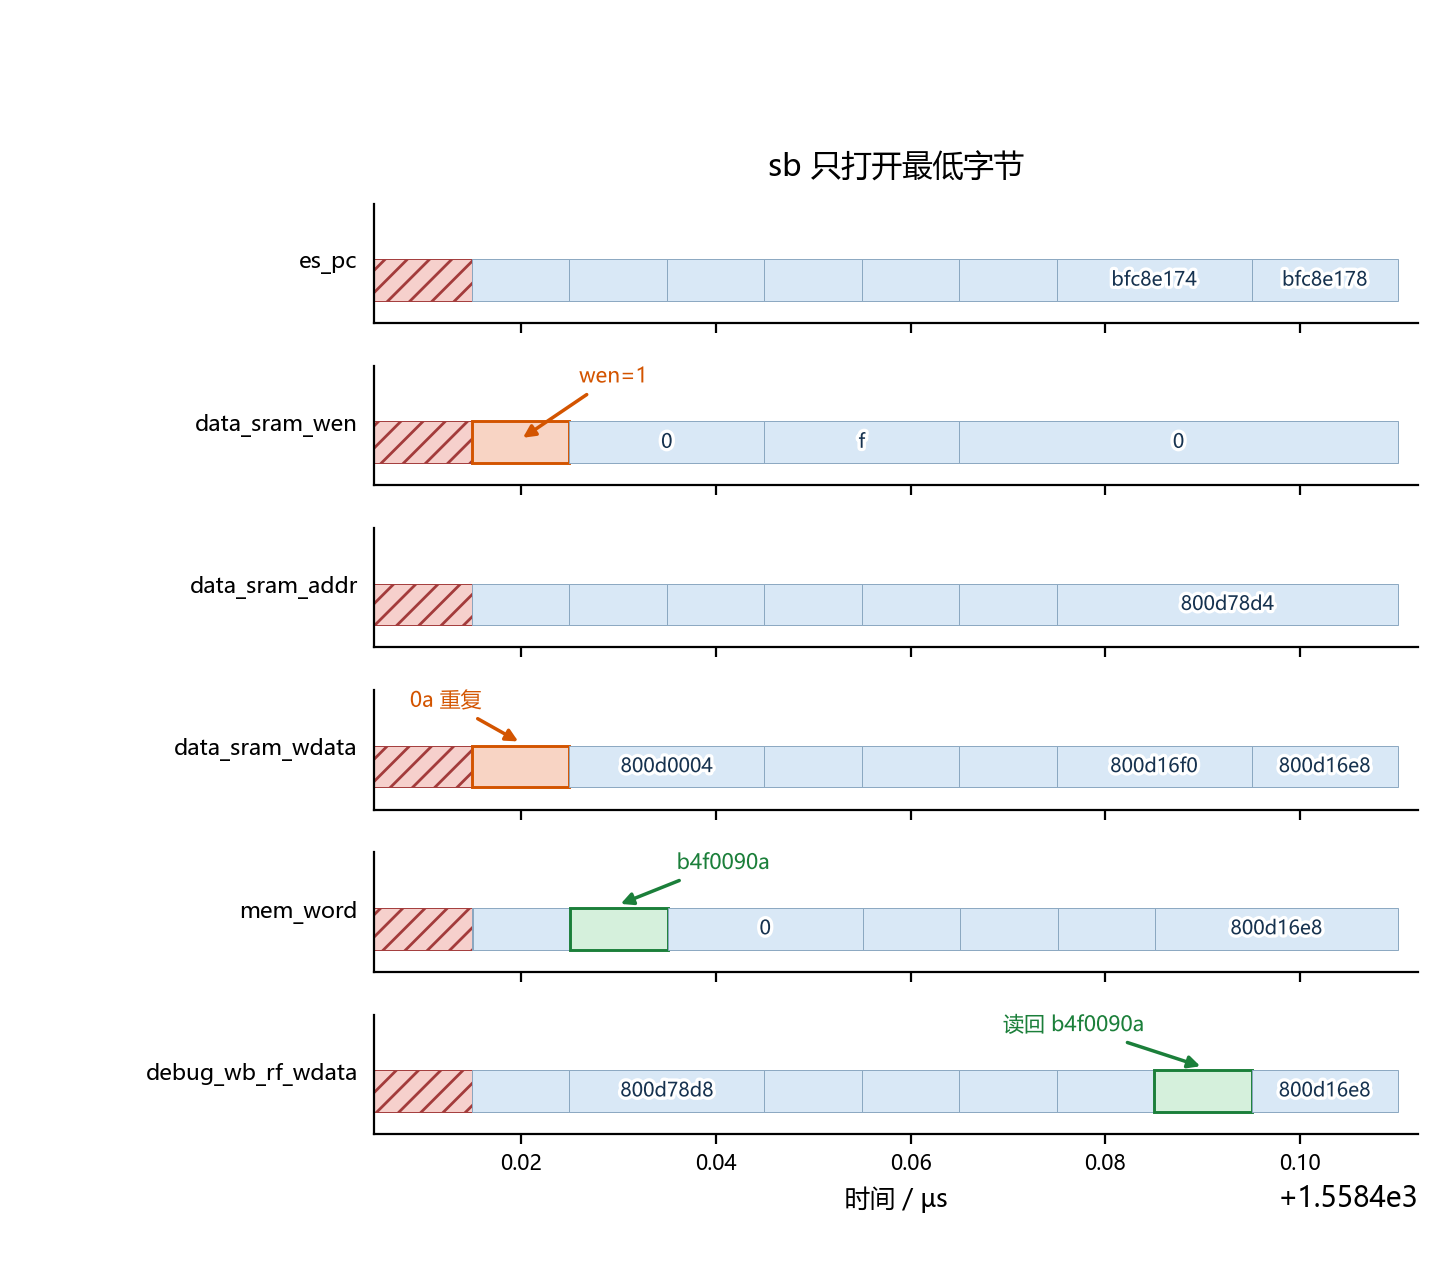
\includegraphics[width=\linewidth]{fig/sb.png}
  \caption{\texttt{sb} 的写使能为 1。内存字变为 \texttt{b4f0090a}，随后 \texttt{lw} 读回该值。}
  \label{fig:sb}
\end{figure}

\section{实验收获}
流水线从实验1的定点算术扩展到乘除、带链接的分支和部分字访存。
立即数按指令选择符号扩展或零扩展，\texttt{SLTIU} 在符号扩展之后做无符号比较。
乘除把结果写入 HI/LO 时让执行级停住，后面的 \texttt{MFHI}/\texttt{MFLO} 读到的是新值。
模块级随机测试里，乘法 991 次与参考值一致；除法的无符号核在 34 拍给出结果，
与测试台原上限重合，上限放宽到 60 拍后 129 次商和余数一致。
\texttt{LWR} 第一次失败时写回只差一个高字节，对照地址低两位和拼接表可以找到被截断的那一段。

\section{附：源码目录}
CPU 仍在实验1的工程里改。\texttt{lab2} 放测试程序、仿真脚本和本报告。
\begin{itemize}
\item \verb|lab1/lab3/CPU_CDE/mycpu_verify/rtl/myCPU/ID_stage.v|
\item \verb|lab1/lab3/CPU_CDE/mycpu_verify/rtl/myCPU/EXE_stage.v|
\item \verb|lab1/lab3/CPU_CDE/mycpu_verify/rtl/myCPU/MEM_stage.v|
\item \verb|lab1/lab3/CPU_CDE/mycpu_verify/rtl/myCPU/mycpu.h|
\item \verb|lab1/lab3/CPU_CDE/mycpu_verify/testbench/mycpu_tb.v|
\item \verb|lab1/lab3/CPU_CDE/cpu132_gettrace/golden_trace.txt|
\item \verb|lab1/lab3/CPU_CDE/soft/func_lab6/obj/inst_ram.coe|
\item \verb|lab1/lab3/CPU_CDE/soft/func_lab7/obj/inst_ram.coe|
\item \verb|lab2/lab6/func_lab6/|
\item \verb|lab2/lab7/func_lab7/|
\item \verb|lab2/lab6/乘法器模块级验证顶层/mul.v|
\item \verb|lab2/lab6/乘法器模块级验证顶层/div.v|
\item \verb|lab2/sim/run_md_tb.tcl|
\item \verb|lab2/sim/run_mycpu_lab6.tcl|
\item \verb|lab2/report/report.tex|
\end{itemize}

\end{document}
